\chapter{Implementation} % (fold)
\label{chap:Implementation}
This chapter introduces the employed protocol specification, the implementation
    of the MEADcast router and sender, as well as the testbed.

\section{Protocol Specification} % (fold)
Since the existing literature on MEADcast lacks specific details regarding the
    header, such as the size of each field, we introduce the
    specifications utilized for our experiments.

Firstly, we omit the usage of an empty Hop-by-Hop IPv6 extension header as
    introduced by \citeauthor{meadcast1} \cite{meadcast1, meadcast2}.
We do this for several reasons:
First, to reduce the overhead of MEADcast.
Second, if a non-MEADcast router attempts to process Hop-by-Hop extension headers
    the packet probably end up in the router's slow path \cite{rfc7045}, potentially
    harming the protocol's performance.
Third, since the MEADcast header is intended to be processed exclusively by
    MEADcast routers, over which we maintain control, the Hop-by-Hop extension
    header serves no purpose.
Lastly, according to various research studies, packets containing a Hop-by-Hop
    extension header experience an increased drop rate of up to 40\% compared
    to packets without an extension header \cite{rfc7872_ext_hdrs_drop_rate},
    especially across multiple \glspl{as} \cite{rfc9098_ext_hdrs_op_impl, rfc9288}.

Next, we introduce the detailed characteristics of the MEADcast header in our
    implementation.
The first four octets of the MEADcast header constitute the static Routing
    extension header, which is shared by all routing variants.
This differs from previous implementations of MEADcast, which omitted the
    Segments Left field \cite{sdn_ba}.
We decided to include this field to comply with RFC 8200
    \cite{rfc8200_ipv6_hdr}, reducing the likelihood that intermediate nodes
    drop MEADcast packets due to a malformed Routing header.
Since there is no existing Routing Type designated for MEADcast, we utilize the
    experimental values of 253 and 254 in accordance with RFC3692
    \cite{rfc3692_ipv6_rt_type}.
The Segments Left field remains fixed to zero and is never altered because,
    according to RFC 8200 \cite{rfc8200_ipv6_hdr}, intermediate nodes that do
    not recognize the employed Routing type value must ignore the Routing
    header and proceed to process the next header.
An illustration of the MEADcast header layout can be found in
    \autoref{lst:meadcast_header}, along with an in-depth description of each
    field in \autoref{tab:meadcast_header}.
Due to the time frame of this thesis, we omit the usage of the optional port
    list as it does not affect the core MEADcast processing.

% No exact definition (size of each field, bit for bit)
% Removed IPv6 Hop-by-Hop header
%   - Reduce Size
%   - Often dropped (cite)
%   - If processed end up in slow path
%   - Only MEADcast router have to process the packet anyway
% Adjusted Routing Header
%   - Invalid routing header in BA (better use valid header)
%   - reduced size
%   - Omitted optional Port List for testing
\label{sec:Protocol Specification}
% python protocol "Next Header:8,Hdr Ext Len:8,Routing Type:8,Num. Dst:8,Flags:2,Hops:6,Reserved:24,Delivery Map:32,Router Map:32,Address List:128"
% python protocol "Next Header:8,Hdr Ext Len:8,Routing Type:8,Segments Left:8,Num. Dst:8,Flags:2,Hops:6,Reserved:16,Delivery Map:32,Router Map:32,Address List:128"

% \begin{figure}[h!]
% \centering
% \begin{lstlisting}[xleftmargin=.07\textwidth]
%  0                   1                   2                   3
%  0 1 2 3 4 5 6 7 8 9 0 1 2 3 4 5 6 7 8 9 0 1 2 3 4 5 6 7 8 9 0 1
% +-+-+-+-+-+-+-+-+-+-+-+-+-+-+-+-+-+-+-+-+-+-+-+-+-+-+-+-+-+-+-+-+
% |  Next Header  |  Hdr Ext Len  |  Routing Type |    Num. Dst   |
% +-+-+-+-+-+-+-+-+-+-+-+-+-+-+-+-+-+-+-+-+-+-+-+-+-+-+-+-+-+-+-+-+
% |Fl.|    Hops   |                    Reserved                   |
% +-+-+-+-+-+-+-+-+-+-+-+-+-+-+-+-+-+-+-+-+-+-+-+-+-+-+-+-+-+-+-+-+
% |                          Delivery Map                         |
% +-+-+-+-+-+-+-+-+-+-+-+-+-+-+-+-+-+-+-+-+-+-+-+-+-+-+-+-+-+-+-+-+
% |                           Router Map                          |
% +-+-+-+-+-+-+-+-+-+-+-+-+-+-+-+-+-+-+-+-+-+-+-+-+-+-+-+-+-+-+-+-+
% |                                                               |
% .                                                               .
% .                          Address List                         .
% .                                                               .
% |                                                               |
% +-+-+-+-+-+-+-+-+-+-+-+-+-+-+-+-+-+-+-+-+-+-+-+-+-+-+-+-+-+-+-+-+
% \end{lstlisting}
% \caption{Python: MEADcast Header}
% \end{figure}

\begin{figure}[!htbp]
\centering
\begin{lstlisting}[xleftmargin=.07\textwidth]
 0                   1                   2                   3
 0 1 2 3 4 5 6 7 8 9 0 1 2 3 4 5 6 7 8 9 0 1 2 3 4 5 6 7 8 9 0 1
+-+-+-+-+-+-+-+-+-+-+-+-+-+-+-+-+-+-+-+-+-+-+-+-+-+-+-+-+-+-+-+-+
|  Next Header  |  Hdr Ext Len  |  Routing Type | Segments Left |
+-+-+-+-+-+-+-+-+-+-+-+-+-+-+-+-+-+-+-+-+-+-+-+-+-+-+-+-+-+-+-+-+
|    Num. Dst   |Fl.|    Hops   |            Reserved           |
+-+-+-+-+-+-+-+-+-+-+-+-+-+-+-+-+-+-+-+-+-+-+-+-+-+-+-+-+-+-+-+-+
|                          Delivery Map                         |
+-+-+-+-+-+-+-+-+-+-+-+-+-+-+-+-+-+-+-+-+-+-+-+-+-+-+-+-+-+-+-+-+
|                           Router Map                          |
+-+-+-+-+-+-+-+-+-+-+-+-+-+-+-+-+-+-+-+-+-+-+-+-+-+-+-+-+-+-+-+-+
|                                                               |
.                                                               .
.                          Address List                         .
.                                                               .
|                                                               |
+-+-+-+-+-+-+-+-+-+-+-+-+-+-+-+-+-+-+-+-+-+-+-+-+-+-+-+-+-+-+-+-+

\end{lstlisting}
\caption{MEADcast header specification}
\label{lst:meadcast_header}
\end{figure}


\bgroup
\begin{table}[!htbp]
\centering
\def\arraystretch{1.35}%  1 is the default
\setlength{\tabcolsep}{1.2em}
\begin{tabularx}{\textwidth}{lX}
\toprule
\textbf{Field}& \textbf{Desciption} \\
\midrule
Next Header   & A 8-bit selector, identifying the type of the immediately
                following header \cite{rfc8200_ipv6_hdr}.
                Employs identical values as the IPv4 Protocol field (e.g. 17 =
                UDP, 59 = No Next Header for IPv6)
                \cite{iana_prot_nums}.\\
Hdr Ext Len   & An 8-bit unsigned integer representing the length of the
                Routing header in 8-octet units, excluding the initial 8
                octets \cite{rfc8200_ipv6_hdr}. \\
Routing Type  & An 8-bit identifier denoting a specific Routing header variant
                \cite{rfc8200_ipv6_hdr}.
                Given the absence of an existing Routing Type for MEADcast, we
                utilize the experimental values of 253 and 254 in accordance
                with RFC3692 \cite{rfc3692_ipv6_rt_type}.\\
Segments Left & An 8-bit unsigned integer representing the number of remaining
                route segments, indicating the number of explicitly listed
                intermediate nodes yet to be traversed before reaching the
                final destination \cite{rfc8200_ipv6_hdr}.
                Remains fixed to zero and is not modified by MEADcast routers.
                Consequently, intermediate nodes that do not recognize the
                employed Routing type value are required to disregard the
                MEADcast header and proceed to process the subsequent header
                \cite{rfc8200_ipv6_hdr}.\\
Num. Dst.     & An 8-bit unsigned integer denoting the number of IPv6
                addresses encoded in the address list.
                The field size sets a theoretical limit of 255 destinations.\\
Flags         & A 2-bit Bitmap. The highest-order bit classifies the packet
                either as a data (0) or discovery  (1) packet.
                The lowest-order bit indicates whether the packet is a
                discovery request (0) or response (1) \cite{meadcast2}.
                Valid combinations comprise \inlinelst{00}, \inlinelst{10}, and
                \inlinelst{11}\\
Hops          & An 6-bit unsigned integer, specifying the distance between the
                sender and a router, denoted in the number of MEADcast hops.
                This field is utilized during the discovery phase. The sender
                initializes the field with zero, and it is incremented by each
                intermediate MEADcast router encountered.
                The field size sets a theoretical limit of 63 hops.\\
Reserved      & A 16-bit reserved field.
                Should be initialized to zero during transmission and
                disregarded upon reception.\\
Delivery Map  & A 32-bit Bitmap, where each bit at position $i$ indicates
                whether a router at index $i$ in the address list has already
                been delivered (0 = delivered, 1 = not yet delivered)
                \cite{meadcast2}. \\
Router Map    & A 32-bit Bitmap, where each bit at position $i$ indicates
                whether an address at index $i$ in the address list is a
                router (0 = receiver, 1 = router) \cite{meadcast2}.\\
Address List  & A variable-length list comprising the IPv6 addresses of
                receivers and MEADcast routers.
                The field size of the Delivery and Router Bitmap imposes a
                practical limit of 32 addresses.\\
\bottomrule
\end{tabularx}
\caption{MEADcast header field description}
\label{tab:meadcast_header}
\end{table}
\egroup

% section Protocol Specification (end)

\section{Router} % (fold)
\label{sec:Router}
This section provides an overview of the MEADcast router implementation in the
    Linux Kernel.
The MEADcast routing software is developed and tested using the latest stable
    Kernel release, version 6.5.3, at the time of development.
MEADcast routing capabilities are tightly coupled to the flow of IPv6 packets
    through the Kernel network stack, making it infeasible to create a separate
    Kernel module loadable at runtime.
Therefore, we decided to extend the IPv6 module with MEADcast capability.
This feature can be enabled or disabled at compile-time using the
    \inlinelst{CONFIG\_IPV6\_MEADCAST} flag.
To avoid the burden of recompiling or switching the kernel to enable or disable
    MEADcast support, we introduce a runtime configuration flag.
This flag is managed through Sysctl, providing the virtual file
    \inlinelst{/proc/sys/net/ipv6/meadcast/enable}, which contains either 0 for
    disabled and 1 for enabled.
For instance, the root user can enable MEADcast support by running the command
    \inlinelst{"echo 1 > /proc/sys/net/ipv6/meadcast/enable"}.
However, it is crucial to ensure that this additional check does not adversely
    impact performance compared to a plain kernel, as it could potentially
    affect the reliability of experimental results.

As illustrated in \autoref{sub:Network Stack}, packets not designated to the
    router itself follow the ``forwarding'' packet flow in the Kernel.
IPv6 extension headers of these packets are normally ignored by the Kernel
    (except for the Router Alert extension).
Consequently, we embedded the entry point for MEADcast processing at the end of
    the \inlinelst{ip6\_forward} method located in
    \inlinelst{net/ipv6/ipv6\_output.c}.
If a packet contains the routing header extension the \inlinelst{mdc\_rcv}
    method located in \inlinelst{net/ipv6/mdcast.c} gets invoked.
This method performs basic sanity checks on the MEADcast header and then
    invokes \inlinelst{mdc\_dcv\_rcv} for discovery and
    \inlinelst{mdc\_data\_rcv} for data packets.

% discovery
% - validation
% - increment hop counter
% - clone socket buffer of incomming packet (discovery response)
% - update dst and src ip of discovery response
\textit{Discovery}: First, discovery packets get validated and the hop counter
    in the MEADcast header is incremented.
To create a discovery response the socket buffer struct of the incoming
    discovery request is cloned.
By this, we solely have to update the IP source and destination field of the
    cloned packet, set the response flag, and perform a routing table lookup
    for the sender's address.
The source IP address of the discovery response is set to the IP address
    associated with the interface returned from the routing lookup.
Lastly, the \inlinelst{dst\_output} method is invoked, dispatching the packet to
    the corresponding layer 2 handler.
The processing of the original packet does not need further handling, as it is
    already correctly done by the default forwarding flow.

\textit{Data}: Data packets undergo several steps upon arrival at the MEADcast
    router.
Firstly, they are validated, and the hop counter in the MEADcast header is
    incremented.
Subsequently, the router iterates over the Delivery and Router Bitmap to
    identify undelivered routers (indices set in both bitmaps).
During this iteration, if the router is not the last undelivered router in the
    sequence, the socket buffer of the original packet is cloned and forwarded
    accordingly.
However, if the router is the last undelivered router, the original packet can
    be forwarded without the need for costly replication.
To determine whether to clone the packet, the routers monitors whether an 
    undelivered router at index $r1$ has a successor (another undelivered
    router) at index $r2$, with $r1 < r2$.
The algorithm's specifics are depicted in \autoref{fig:router_hdr_parsing}.

For each undelivered router $R_u$ specified in the MEADcast header, the
    processing router $R_p$ decides whether to transmit the data via MEADcast
    or IP unicast.
If the IP address of $R_u$ in the MEADcast header belongs to the processing
    router $R_p$ itself, all designated endpoints will be delivered via IP
    unicast.
Additionally, if the number of endpoints assigned to the considered router
    $R_u$ from the MEADcast header is below a certain threshold, the processing
    router $R_p$ performs a premature MEADcast to IP unicast transformation.
For example, if $R_u$ has one designated endpoint, $R_p$ could execute a
    premature MEADcast to IP unicast transformation, potentially enhancing
    performance.
The threshold can also be configured during runtime by setting the parameter
    \inlinelst{/proc/sys/net/ipv6/meadcast/min_dsts}.
Setting \inlinelst{min_dsts} to 0 disables premature MEADcast to IP unicast
    transformation.

If the packet is forwarded via MEADcast, the router updates both the delivery
    bitmap and the destination field of the IPv6 header.
In the delivery bitmap, all bits are set to zero except for the index
    corresponding to the considered router.
Additionally, the IP destination field is set to the address of the first
    receiver following the router in the address list.
Lastly, the router performs a routing table lookup for the new destination
    address and forwards the packet accordingly.

In case of IP unicast transmission, the router converts the MEADcast packet
    into an IPv6 packet by copying the IPv6 header in front of the Layer 4
    header and adjusting the socket buffer pointers accordingly.
Additionally, the L4 checksum is corrected due to the modified destination IP
    address.

% Search for first router
%
% - validation
% - increment hop count
% - iterate bitmaps
%   - check which routers aren't delivered yet
%   - if router is not last undelivered router create a copy of socket buffer struct
%   - else use incoming one
% - forwarding
%   - if router addr in bitmap is of router or less than min_dsts eps -> m2u
%   - else: update bitmap (set all others to delivered), update ip dst field
% - m2u
%   - copy IP hdr in front of l3 header
%   - update skb pointers
%   - recalc checksum
\begin{figure}
    \begin{center}
        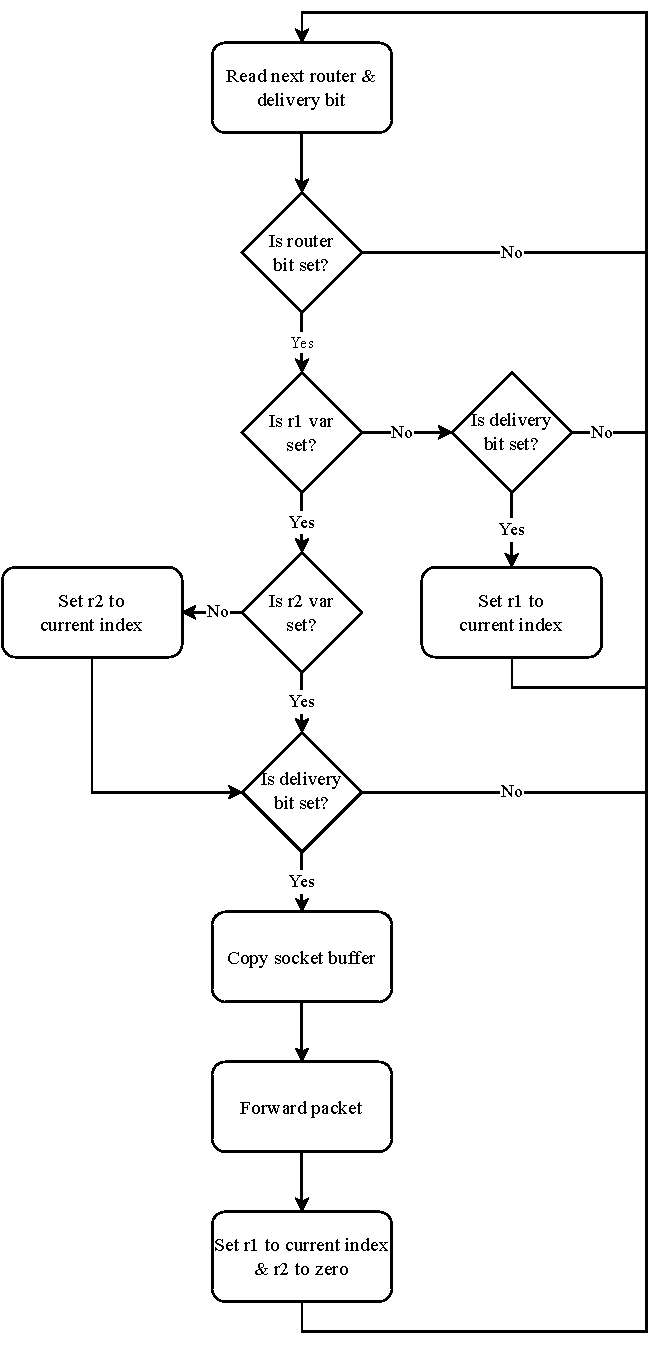
\includegraphics[scale=1]{router_hdr_parsing.pdf}
    \end{center}
    \caption{Router header parsing}
    \label{fig:router_hdr_parsing}
\end{figure}

\begin{figure}
    \begin{center}
        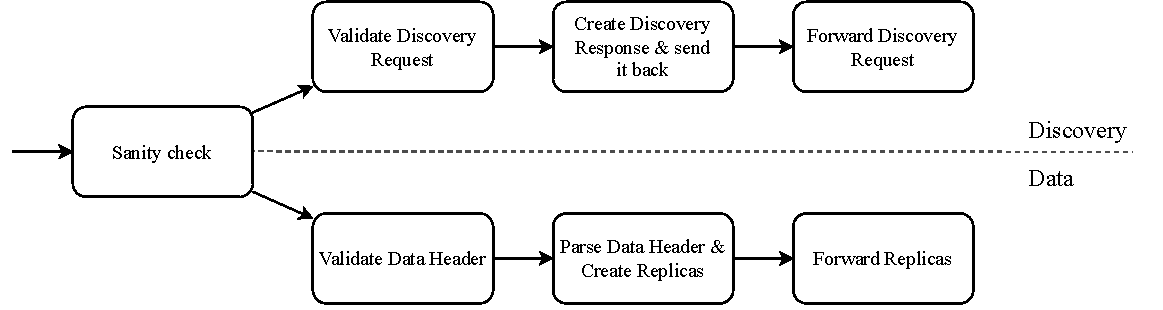
\includegraphics[width=\textwidth]{router_procedure.pdf}
    \end{center}
    \caption{MEADcast router procedure}
    \label{fig:router_procedure}
\end{figure}
% section Router (end)


\section{Sender} % (fold)
\label{sec:Sender}
This section provides an overview of our MEADcast sender implementation.
To ensure an efficient implementation that is comparable to existing network
    protocol implementations, we chose to implement the sender in the C
    language.
The main tasks of the sender include sending periodical discovery requests to
    all group members, receiving discovery responses, constructing a topology
    tree based on the received discovery responses, heuristically grouping
    receivers into MEADcast packets, and transmitting data to all group members
    either via MEADcast or IP unicast.

\paragraph{Startup} % (fold)
\label{par:Startup}
All receivers must be known at startup, dynamic runtime memberships are not
    supported.
We regard this decision as justifiable, given that MEADcast does not define any
    mechanism for joining or leaving a group, and the primary objective of this
    thesis is to compare the protocol with existing alternatives.
On startup the sender initializes a topology tree with itself as the root and
    all receivers as direct attached leafs.
Moreover, a TUN interface is created, which is used as a common interface to
    other applications.
Any data, which is send to the TUN interface will be transmitted to the
    MEADcast group.
The \gls{mtu} of the TUN interface will be set to the MTU of the bind interface
    minus the maximum allowed MEADcast header size.
This ensures, that all packets read from the TUN interface can be transmitted
    via MEADcast.
Additionally, a host route to the TUN interface gets created (default:
    \inlinelst{fd15::1}).
Next, a discovery and transmission thread is created.
This is required to simultaneously transmit data and discovery requests and
    responses.

% Discovery
% - Send and receive discovery
% - Perform grouping
% - Timers

% Transmit
% - Init txg struct (atomic pointer)
% - Read data from TUN & send it to groups

% paragraph Startup (end)
% Startup
% - Create TUN dev (set MTU, set Route)
% - txg only struct shared between threads
% - Implemented in C (efficiency & comparable to other protocols)
% - TUN
% - Automatically set route & MTU
% - Judy Array to quickly find IPs
% - Tree for grouping
% - grouping algorithm
% section Sender (end)


\section{Testbed} % (fold)
\label{sec:Testbed_Implementation}
% - python script reading json
% - kvm, direct kernel boot, debian nocloud image
% - chrony time sync (had to change boot param on host system)
% section Testbed (end)


% chapter Implementation (end)
